\documentclass[xcolor={dvipsnames}]{beamer}

% \usepackage{lmodern}
\usepackage[utf8]{inputenc}
\usepackage{lmodern}
\usepackage{amssymb, amsmath, amsthm, graphicx}
\usepackage{tikz}
\usepackage{pgfplots}
\pgfplotsset{compat=1.9}

\usetheme{Frankfurt}
\renewcommand{\phi}{\varphi}
\renewcommand{\epsilon}{\varepsilon}
\newcommand{\df}[1]{\textcolor{BrickRed}{\emph{#1}}}
\renewcommand{\th}[1]{\textcolor{Fuchsia}{\emph{#1}}}
\renewcommand{\hat}{\widehat}

\newcommand{\cD}{\mathcal{D}}
\newcommand{\cL}{\mathcal{L}}
\newcommand{\cM}{\mathcal{M}}
\newcommand{\cN}{\mathcal{N}}
\newcommand{\cX}{\mathcal{X}}
\newcommand{\cZ}{\mathcal{Z}}
\newcommand{\EE}{\mathbb{E}}
\newcommand{\vv}{\mathbf{v}}
\newcommand{\vw}{\mathbf{w}}
\newcommand{\vx}{\mathbf{x}}
\newcommand{\vy}{\mathbf{y}}
\newcommand{\vY}{\mathbf{Y}}
\newcommand{\One}{\mathbf{1}}
\newcommand{\vbeta}{\boldsymbol{\beta}}


\newcommand{\RR}{\mathbb{R}}

\newcommand{\train}{{\text{train}}}
\newcommand{\test}{{\text{test}}}

\DeclareMathOperator*{\argmin}{argmin}
\DeclareMathOperator{\Bias}{Bias}
\DeclareMathOperator{\Var}{Var}
\DeclareMathOperator{\MSE}{MSE}
\DeclareMathOperator{\MISE}{MISE}
\DeclareMathOperator{\Bernoulli}{Bernoulli}

\title[DATA 607]{DATA 607 Statistical and Machine Learning\\
\textit{Session 3: Kernel Smoothers;\\Nonparametric Classifiers}}
\author{Matthew Greenberg}
\institute[]{Department of Mathematics and Statistics\\
University of Calgary}
\date{22.03.2020}



% \includeonlyframes{current}

\begin{document}

\frame{\titlepage}

\begin{frame}{This Evening's Agenda}
    \setlength\parskip{0.75em}
    \tableofcontents
\end{frame}

\begin{frame}
    \frametitle{Indicator Functions}
    \setlength\parskip{0.75em}

    Define the \textbf{Boxcar Kernel} by
    \[
        B(x) = \begin{cases}
            \frac12&\text{if $-1<x<1$,}\\
            0&\text{otherwise.}
        \end{cases}\qquad (\vx\in\RR).
    \]

    \begin{center}
    \begin{tikzpicture}
        \draw (0, -0.5) -- (0, 1.5);
        \draw (-0.15, 1) node[above left] {$\frac12$} -- (0.15, 1);
        \draw (-3.8, 0) -- (3.8, 0);
        \draw (-1, 0.15) -- (-1, -0.15) node[below] {$-1$};
        \draw (1, 0.15) -- (1, -0.15) node[below] {$1$};
        \draw[very thick, blue] (-3.8, 0) -- (-1, 0) -- (-1, 1) -- (1, 1) -- (1, 0)
        -- (3.8, 0) node[black, above right] {$y=B(x)$};

        % \begin{scope}[yshift=-2.5cm]
        %     \draw (0, -0.5) -- (0, 1.5);
        %     \draw (-0.15, 1) node[left] {$\frac12$} -- (0.15, 1);
        %     \draw (-3.8, 0) -- (3.8, 0);
        %     \draw (1, 0.15) -- (1, -0.15) node[below] {$1$};
        %     \draw (2, 0.15) -- (2, -0.15) node[below] {$2$};
        %     \draw (3, 0.15) -- (3, -0.15) node[below] {$3$};
        %     \draw[very thick, blue] (-3.8, 0) -- (1, 0) -- (1, 1) -- (3, 1) -- (3, 0) --
        %     (3.8, 0) node[black, above right] {$y=B(x-2)$};
        % \end{scope}
        \end{tikzpicture}
        \end{center}
\end{frame}

\begin{frame}
    \frametitle{Sliding Window Smoother}
    \setlength\parskip{0.75em}

    \textbf{Data set:}
    \[
        \cD = \{(\vx_1,y_1),\;(\vx_1,y_1),\;\ldots,\;(\vx_n, y_n)\}
    \]
    
    \textbf{Boxcar Kernel Smoother:}
    \[
    \hat r_{h,\cD}(\vx) = \frac{\displaystyle\quad\sum_{i=1}^n y_i\,B\left(\frac{\vx - \vx_i}h\right)\quad}    
    {\displaystyle\sum_{i=1}^n B\left(\frac{\vx - \vx_i}h\right)}
    %\hat r_{h,\cD}(\vx) = \frac1{\# I(\vx)}\sum_{i\in I(\vx)} y_i
    \]
    \textbf{Generalization:} Replace $B$ by different ``kernel'' function.
\end{frame}

\begin{frame}
\begin{align*}
B\left(\frac{x_i - x}h\right) &= \begin{cases}
    1&\text{if $-1<\dfrac{x_i-x}h$}<1\\[1ex]
    0&\text{otherwise}
\end{cases}\\[1ex]
&= \begin{cases}
    1&\text{if $-h<x_i-x<h$}\\[1ex]
    0&\text{otherwise}
\end{cases}\\[1ex]
&= \begin{cases}
    1&\text{if $x-h<x_i<x+h$}\\[1ex]
    0&\text{otherwise}
\end{cases}
\end{align*}
    
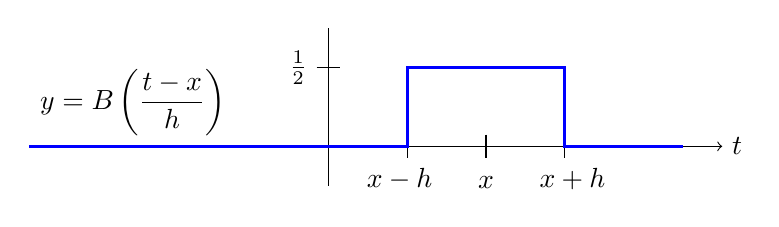
\begin{tikzpicture}
            \draw (0, -0.5) -- (0, 1.5);
            \draw (-0.15, 1) node[left] {$\frac12$} -- (0.15, 1);
            \draw[->] (-3.8, 0) -- (5, 0) node[right] {$t$};
            \draw (1, 0.15) -- (1, -0.15) node[below] {$x-h\;\;$};
            \draw (2, 0.15) -- (2, -0.15);
            \node at (2, -0.46) {$x$};
            \draw (3, 0.15) -- (3, -0.15) node[below] {$\;\;x+h$};
            \draw[very thick, blue] (-3.8, 0)  node[black, above right] {$y=B\left(\dfrac{t-x}h\right)$}-- (1, 0) -- (1, 1) -- (3, 1) -- (3, 0) --
            (4.5, 0);
\end{tikzpicture}
\end{frame}

\begin{frame}
\begin{align*}
    \sum_{i=1}^n B\left(\frac{x_i - x}h\right) &= \text{\# of $x_i$ such that $x-h < x_i < x+h$}
\end{align*}
    

\end{frame}

\begin{frame}
    \frametitle{Kernel Functions}
    \setlength\parskip{0.75em}

    $K(\vx)$ is a \textbf{kernel function} if
    \begin{enumerate}
        \setlength\parskip{0.75em}
        \item $K(\vx)\geq 0$
        \item $K(-\vx)=K(\vx)$
        \item $\displaystyle \int_{\RR^n}K(\vx)d\vx = 1$
    \end{enumerate}
\end{frame}

\begin{frame}
    \frametitle{Popular Kernels}
    \begin{enumerate}
        \setlength\parskip{0.75em}
        \item Boxcar: $$B(x) = \dfrac12\One_{(-1, 1)}(x)$$
        \item Triangular: $$T(x) = (1 - |x|)\One_{(-1, 1)}(x)$$
        \item Epanechnikov: $$E(x) = \dfrac34(1-x^2)\One_{(-1, 1)}(x)$$
        \item Gaussian: $$G(x) = \dfrac1{\sqrt{2\pi}}e^{-x^2/2}$$
    \end{enumerate}
\end{frame}

\begin{frame}
    \frametitle{Popular Kernels}
    \begin{center}
    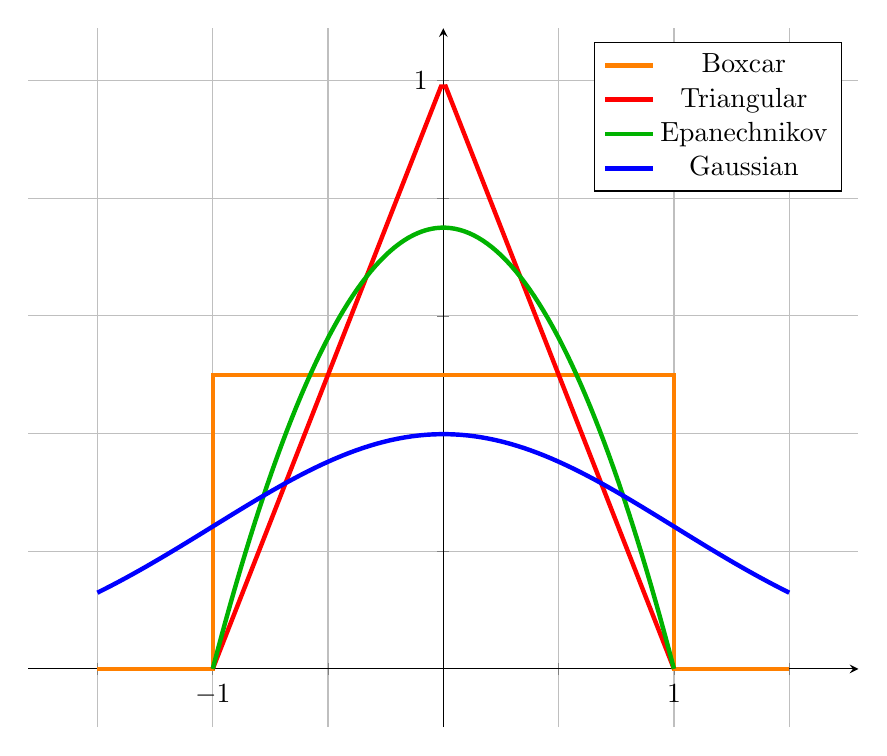
\begin{tikzpicture}
        \begin{axis}[grid=both,
                    axis lines=middle,
                    width=\textwidth,
                    xtick={-1.5, -1, -0.5, 0, 0.5, 1, 1.5},
                    xticklabels={{}, $-1$, {}, {}, {}, $1$},
                    ytick={0.2, 0.4, 0.6, 0.8, 1},
                    yticklabels={{}, {}, {}, {}, $1$},
                    enlargelimits]

        \addplot[orange, ultra thick] coordinates {
            (-1.5,0)
            (-1,0)
            (-1,0.5)
            (1,0.5)
            (1,0)
            (1.5, 0)
        };
        \addlegendentry{Boxcar};

        \addplot[red, ultra thick, domain=-1:1, samples=100]  {1 - abs(x)};
        \addlegendentry{Triangular};

        \addplot[black!30!green, ultra thick, domain=-1:1, samples=100]  {3*(1-x^2)/4};
        \addlegendentry{Epanechnikov};

        \addplot[blue, ultra thick, domain=-1.5:1.5, samples=100]  {exp(-x^2/2)/sqrt(2*pi)};
        \addlegendentry{Gaussian};
        \end{axis}
    \end{tikzpicture}
\end{center}

\end{frame}

\end{document}